The main interest of interactive simulation is that the user can modify the course of the computations in real-time.
This is essential for surgical simulation : during a training procedure, when a virtual medical instrument comes into contact with some models of a soft-tissue, \emph{instantaneous} deformations must be computed.
This visual feedback of the contact can be enhanced by haptic rendering so that the surgeon can really "feel" the contact.

There are two main issues for a platform like SOFA for providing haptic: The first is that haptic forces need to be computed at $1kHz$ whereas real-time visual feedback (without haptic) is obtained at $30Hz$. The second is that haptic feedback can add artificially some energy inside the simulation and can create instabilities, if the control is not \emph{passive}. 

Thus two different approaches are currently implemented into SOFA. The first one is the \emph{Virtual Coupling} technique and the other, more advanced, allows for rendering the constraints presented in section \ref{lm}.



\section{Virtual Coupling} Plugging of a haptic device is bidirectional: the user applies some motions or some forces on the device and this device, in return, applies forces and/or motions to the user.
The majority of the haptic devices propose a \emph{Impedance} coupling: the position of the device is provided by the API and this API asks for force values from the application.
A very simple scheme of coupling, presented in Fig\ref{fig:haptic1}, could have been used.
In this \emph{Direct coupling} case, the simulation would play the role of a controller in an open loop. 

\begin{figure}
\centering
 
\includegraphics[width=0.7\linewidth]{haptic1.png}
 \caption{Direct coupling}
 \label{fig:haptic1}
\end{figure}

Such design is not suitable when stable and robust haptic feedback on a virtual environment is desired. Indeed some combination of the environment impedance and human user reactions can destabilize the system \cite{Adams99}. 
To avoid this, a virtual mechanical coupling is set. It corresponds to the use of a damped-stiffness between the position measured on the device and the simulated position in the virtual environment (see Fig\ref{fig:haptic2}). If very stiff constraints are being simulated then, the stiffness perceived by the user will not be infinite but will correspond to the stiffness of this virtual coupling. 
Hence, a compromise between stability and performance must be found by tuning the stiffness value of the coupling.

\begin{figure}
\centering
 
\includegraphics[width=\linewidth]{haptic2.png}
 \caption{Virtual coupling technique. A 6 DoFs Damped spring is placed between the haptic loop and the simulation.}
 \label{fig:haptic2}
\end{figure}

The damped spring is simulated two times. One time in the haptic loop and one time in the simulation loop. 
If the two loops are synchronized, then the result is the same. But it can also be used in asynchronous mode: fast update of the haptic loop and low rates in the simulation.
In such case, the haptic feedback remains stable but the delay between the two loop is creating an artificial damping.
There is an option to cancel this artificial damping if no contact is detected in the simulation. However, this option can create a sensation of sticking contacts. 
The main advantage of the virtual coupling technique is that it can be easily employed with every simulation of SOFA. The main drawback is that the haptic rendering is not transparent.
 
\section{Constraint-based rendering} An innovative way of dealing with haptic rendering for medical simulation has been proposed in the context of SOFA (see\footnote{The implementation of  \cite{Saupin08} is available in open-source, for the implementation of \cite{Peterlik11}, please contact: christian.duriez@inria.fr }  \cite{Saupin08} and \cite{Peterlik11}). 
The approach deals with the mechanical interactions using appropriate force and/or motion transmission models named \emph{compliant mechanisms} (see Fig\ref{fig:haptic3}). 
These mechanisms are formulated as a constraint-based problem (like presented in section \ref{lm}) that is solved in two separate threads running at different frequencies. 
The first thread processes the whole simulation including the soft-tissue deformations, whereas the second one only deals with computer haptics. 
With this approach, it is possible to describe the specific behavior of various medical devices while relying on a unified method for solving the mechanical interactions between deformable objects and haptic rendering.  
\begin{figure}
\centering
 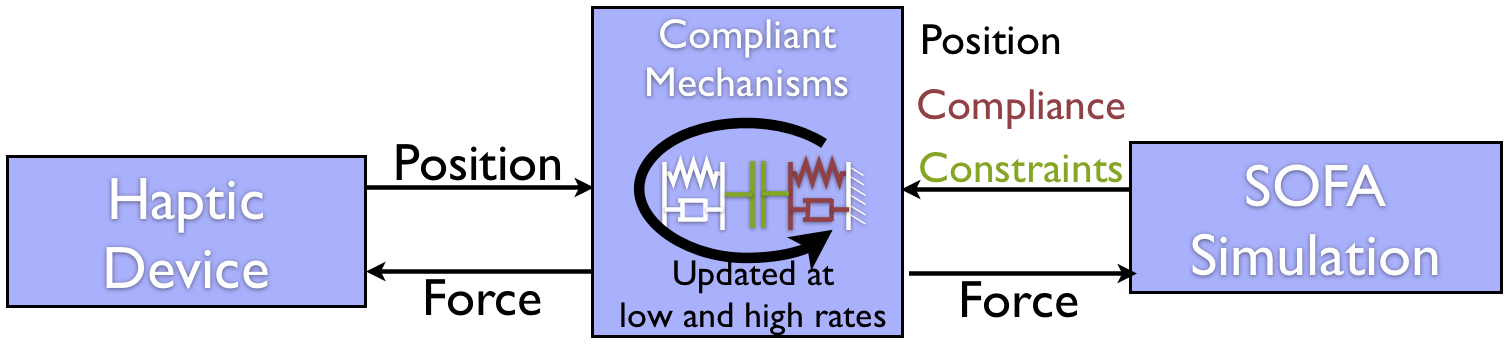
\includegraphics[width=\linewidth]{haptic3.png}
 \caption{Compliant mechanisms technique. The simulation shares the mechanical compliance of the objects and the constraints between them. The constraint response is being computed at low rate within the simulation and at high rates within a separate haptic thread. A 6 DoFs Damped spring is still used to coupled the position of the device to its position in the simulation}
 \label{fig:haptic3}
\end{figure}

\section{How to use it in SOFA ?}
Please see the web page: http://wiki.sofa-framework.org/wiki/Haptic  and use the tutorial "dentistry".

